\documentclass[]{article}
\usepackage{lmodern}
\usepackage{amssymb,amsmath}
\usepackage{ifxetex,ifluatex}
\usepackage{fixltx2e} % provides \textsubscript
\ifnum 0\ifxetex 1\fi\ifluatex 1\fi=0 % if pdftex
  \usepackage[T1]{fontenc}
  \usepackage[utf8]{inputenc}
\else % if luatex or xelatex
  \ifxetex
    \usepackage{mathspec}
  \else
    \usepackage{fontspec}
  \fi
  \defaultfontfeatures{Ligatures=TeX,Scale=MatchLowercase}
\fi
% use upquote if available, for straight quotes in verbatim environments
\IfFileExists{upquote.sty}{\usepackage{upquote}}{}
% use microtype if available
\IfFileExists{microtype.sty}{%
\usepackage{microtype}
\UseMicrotypeSet[protrusion]{basicmath} % disable protrusion for tt fonts
}{}
\usepackage[margin=1in]{geometry}
\usepackage{hyperref}
\hypersetup{unicode=true,
            pdftitle={Homework12},
            pdfauthor={Jorge Ruiz Arocho},
            pdfborder={0 0 0},
            breaklinks=true}
\urlstyle{same}  % don't use monospace font for urls
\usepackage{color}
\usepackage{fancyvrb}
\newcommand{\VerbBar}{|}
\newcommand{\VERB}{\Verb[commandchars=\\\{\}]}
\DefineVerbatimEnvironment{Highlighting}{Verbatim}{commandchars=\\\{\}}
% Add ',fontsize=\small' for more characters per line
\usepackage{framed}
\definecolor{shadecolor}{RGB}{248,248,248}
\newenvironment{Shaded}{\begin{snugshade}}{\end{snugshade}}
\newcommand{\KeywordTok}[1]{\textcolor[rgb]{0.13,0.29,0.53}{\textbf{#1}}}
\newcommand{\DataTypeTok}[1]{\textcolor[rgb]{0.13,0.29,0.53}{#1}}
\newcommand{\DecValTok}[1]{\textcolor[rgb]{0.00,0.00,0.81}{#1}}
\newcommand{\BaseNTok}[1]{\textcolor[rgb]{0.00,0.00,0.81}{#1}}
\newcommand{\FloatTok}[1]{\textcolor[rgb]{0.00,0.00,0.81}{#1}}
\newcommand{\ConstantTok}[1]{\textcolor[rgb]{0.00,0.00,0.00}{#1}}
\newcommand{\CharTok}[1]{\textcolor[rgb]{0.31,0.60,0.02}{#1}}
\newcommand{\SpecialCharTok}[1]{\textcolor[rgb]{0.00,0.00,0.00}{#1}}
\newcommand{\StringTok}[1]{\textcolor[rgb]{0.31,0.60,0.02}{#1}}
\newcommand{\VerbatimStringTok}[1]{\textcolor[rgb]{0.31,0.60,0.02}{#1}}
\newcommand{\SpecialStringTok}[1]{\textcolor[rgb]{0.31,0.60,0.02}{#1}}
\newcommand{\ImportTok}[1]{#1}
\newcommand{\CommentTok}[1]{\textcolor[rgb]{0.56,0.35,0.01}{\textit{#1}}}
\newcommand{\DocumentationTok}[1]{\textcolor[rgb]{0.56,0.35,0.01}{\textbf{\textit{#1}}}}
\newcommand{\AnnotationTok}[1]{\textcolor[rgb]{0.56,0.35,0.01}{\textbf{\textit{#1}}}}
\newcommand{\CommentVarTok}[1]{\textcolor[rgb]{0.56,0.35,0.01}{\textbf{\textit{#1}}}}
\newcommand{\OtherTok}[1]{\textcolor[rgb]{0.56,0.35,0.01}{#1}}
\newcommand{\FunctionTok}[1]{\textcolor[rgb]{0.00,0.00,0.00}{#1}}
\newcommand{\VariableTok}[1]{\textcolor[rgb]{0.00,0.00,0.00}{#1}}
\newcommand{\ControlFlowTok}[1]{\textcolor[rgb]{0.13,0.29,0.53}{\textbf{#1}}}
\newcommand{\OperatorTok}[1]{\textcolor[rgb]{0.81,0.36,0.00}{\textbf{#1}}}
\newcommand{\BuiltInTok}[1]{#1}
\newcommand{\ExtensionTok}[1]{#1}
\newcommand{\PreprocessorTok}[1]{\textcolor[rgb]{0.56,0.35,0.01}{\textit{#1}}}
\newcommand{\AttributeTok}[1]{\textcolor[rgb]{0.77,0.63,0.00}{#1}}
\newcommand{\RegionMarkerTok}[1]{#1}
\newcommand{\InformationTok}[1]{\textcolor[rgb]{0.56,0.35,0.01}{\textbf{\textit{#1}}}}
\newcommand{\WarningTok}[1]{\textcolor[rgb]{0.56,0.35,0.01}{\textbf{\textit{#1}}}}
\newcommand{\AlertTok}[1]{\textcolor[rgb]{0.94,0.16,0.16}{#1}}
\newcommand{\ErrorTok}[1]{\textcolor[rgb]{0.64,0.00,0.00}{\textbf{#1}}}
\newcommand{\NormalTok}[1]{#1}
\usepackage{graphicx,grffile}
\makeatletter
\def\maxwidth{\ifdim\Gin@nat@width>\linewidth\linewidth\else\Gin@nat@width\fi}
\def\maxheight{\ifdim\Gin@nat@height>\textheight\textheight\else\Gin@nat@height\fi}
\makeatother
% Scale images if necessary, so that they will not overflow the page
% margins by default, and it is still possible to overwrite the defaults
% using explicit options in \includegraphics[width, height, ...]{}
\setkeys{Gin}{width=\maxwidth,height=\maxheight,keepaspectratio}
\IfFileExists{parskip.sty}{%
\usepackage{parskip}
}{% else
\setlength{\parindent}{0pt}
\setlength{\parskip}{6pt plus 2pt minus 1pt}
}
\setlength{\emergencystretch}{3em}  % prevent overfull lines
\providecommand{\tightlist}{%
  \setlength{\itemsep}{0pt}\setlength{\parskip}{0pt}}
\setcounter{secnumdepth}{0}
% Redefines (sub)paragraphs to behave more like sections
\ifx\paragraph\undefined\else
\let\oldparagraph\paragraph
\renewcommand{\paragraph}[1]{\oldparagraph{#1}\mbox{}}
\fi
\ifx\subparagraph\undefined\else
\let\oldsubparagraph\subparagraph
\renewcommand{\subparagraph}[1]{\oldsubparagraph{#1}\mbox{}}
\fi

%%% Use protect on footnotes to avoid problems with footnotes in titles
\let\rmarkdownfootnote\footnote%
\def\footnote{\protect\rmarkdownfootnote}

%%% Change title format to be more compact
\usepackage{titling}

% Create subtitle command for use in maketitle
\newcommand{\subtitle}[1]{
  \posttitle{
    \begin{center}\large#1\end{center}
    }
}

\setlength{\droptitle}{-2em}
  \title{Homework12}
  \pretitle{\vspace{\droptitle}\centering\huge}
  \posttitle{\par}
  \author{Jorge Ruiz Arocho}
  \preauthor{\centering\large\emph}
  \postauthor{\par}
  \predate{\centering\large\emph}
  \postdate{\par}
  \date{2018 M04 11}


\begin{document}
\maketitle

\section{GGPLOT GRAPHING}\label{ggplot-graphing}

\begin{Shaded}
\begin{Highlighting}[]
\KeywordTok{library}\NormalTok{(ggmap)}
\end{Highlighting}
\end{Shaded}

\begin{verbatim}
## Warning: package 'ggmap' was built under R version 3.4.4
\end{verbatim}

\begin{verbatim}
## Loading required package: ggplot2
\end{verbatim}

\begin{Shaded}
\begin{Highlighting}[]
\KeywordTok{library}\NormalTok{(ggplot2)}
\end{Highlighting}
\end{Shaded}

\begin{Shaded}
\begin{Highlighting}[]
\CommentTok{# I will be using an R dataset package named "PREarthquakes", from the University of Puerto Rico, Mayaguez Campus (my previous college). }
\CommentTok{# This dataset includes the location of seismic events of near the island.}

\NormalTok{PR_Earthquakes =}\StringTok{ }\KeywordTok{read.table}\NormalTok{(}\StringTok{"PREarthquakes.csv"}\NormalTok{, }\DataTypeTok{header=}\OtherTok{TRUE}\NormalTok{,}\DataTypeTok{sep=}\StringTok{","}\NormalTok{, }\DataTypeTok{stringsAsFactors=}\OtherTok{FALSE}\NormalTok{)}
\KeywordTok{head}\NormalTok{(PR_Earthquakes)}
\end{Highlighting}
\end{Shaded}

\begin{verbatim}
##   Magnitude Agency Latitude Longitude Depth Felt
## 1      3.66   PRSN  18.1948  -67.8873   123   No
## 2      3.83   PRSN  18.1026  -68.7711   156   No
## 3      3.47   PRSN  18.9903  -64.9226    26   No
## 4      3.61   PRSN  17.9721  -68.7251   101   No
## 5      3.68   PRSN  18.7591  -68.6516   144   No
## 6      3.58   PRSN  19.2351  -64.8130    28   No
##                       Region
## 1               MONA PASSAGE
## 2 EASTERN DOMINICAN REPUBLIC
## 3      SOMBRERO SEISMIC ZONE
## 4 EASTERN DOMINICAN REPUBLIC
## 5 EASTERN DOMINICAN REPUBLIC
## 6      SOMBRERO SEISMIC ZONE
\end{verbatim}

\begin{Shaded}
\begin{Highlighting}[]
\KeywordTok{names}\NormalTok{(PR_Earthquakes)}
\end{Highlighting}
\end{Shaded}

\begin{verbatim}
## [1] "Magnitude" "Agency"    "Latitude"  "Longitude" "Depth"     "Felt"     
## [7] "Region"
\end{verbatim}

\begin{Shaded}
\begin{Highlighting}[]
\KeywordTok{str}\NormalTok{(PR_Earthquakes)}
\end{Highlighting}
\end{Shaded}

\begin{verbatim}
## 'data.frame':    50 obs. of  7 variables:
##  $ Magnitude: num  3.66 3.83 3.47 3.61 3.68 3.58 3.9 3.46 3.56 3.64 ...
##  $ Agency   : chr  "PRSN" "PRSN" "PRSN" "PRSN" ...
##  $ Latitude : num  18.2 18.1 19 18 18.8 ...
##  $ Longitude: num  -67.9 -68.8 -64.9 -68.7 -68.7 ...
##  $ Depth    : int  123 156 26 101 144 28 9 126 29 33 ...
##  $ Felt     : chr  "No" "No" "No" "No" ...
##  $ Region   : chr  "MONA PASSAGE" "EASTERN DOMINICAN REPUBLIC" "SOMBRERO SEISMIC ZONE" "EASTERN DOMINICAN REPUBLIC" ...
\end{verbatim}

\begin{Shaded}
\begin{Highlighting}[]
\CommentTok{# Now we I am going to create a new dataset that only includes the information that }
\CommentTok{# I will be using (the longitude, latitude and the magnitude) for my maps. }

\NormalTok{Earthquakes =}\StringTok{ }\NormalTok{PR_Earthquakes[}\KeywordTok{c}\NormalTok{(}\StringTok{"Longitude"}\NormalTok{, }\StringTok{"Latitude"}\NormalTok{, }\StringTok{"Magnitude"}\NormalTok{)]}
\KeywordTok{head}\NormalTok{(Earthquakes) }\CommentTok{#To verify we will look to the first part of the data. }
\end{Highlighting}
\end{Shaded}

\begin{verbatim}
##   Longitude Latitude Magnitude
## 1  -67.8873  18.1948      3.66
## 2  -68.7711  18.1026      3.83
## 3  -64.9226  18.9903      3.47
## 4  -68.7251  17.9721      3.61
## 5  -68.6516  18.7591      3.68
## 6  -64.8130  19.2351      3.58
\end{verbatim}

\begin{Shaded}
\begin{Highlighting}[]
\NormalTok{PRMap =}\StringTok{ }\KeywordTok{get_map}\NormalTok{(}\DataTypeTok{location=}\StringTok{'puerto rico'}\NormalTok{, }\DataTypeTok{zoom =} \DecValTok{7}\NormalTok{, }\DataTypeTok{maptype =} \StringTok{"satellite"}\NormalTok{, }\DataTypeTok{source =} \StringTok{'google'}\NormalTok{, }\DataTypeTok{color =} \StringTok{'color'}\NormalTok{)}
\end{Highlighting}
\end{Shaded}

\begin{verbatim}
## Map from URL : http://maps.googleapis.com/maps/api/staticmap?center=puerto+rico&zoom=7&size=640x640&scale=2&maptype=satellite&language=en-EN&sensor=false
\end{verbatim}

\begin{verbatim}
## Information from URL : http://maps.googleapis.com/maps/api/geocode/json?address=puerto%20rico&sensor=false
\end{verbatim}

\begin{Shaded}
\begin{Highlighting}[]
\CommentTok{#Once the get_map function has found the map I will combine the ggmap package with }
\CommentTok{#the ggplot2 package. }

\KeywordTok{ggmap}\NormalTok{(PRMap) }\OperatorTok{+}\StringTok{ }\KeywordTok{geom_point}\NormalTok{(}\KeywordTok{aes}\NormalTok{(}\DataTypeTok{x=}\NormalTok{Longitude, }\DataTypeTok{y=}\NormalTok{Latitude, }\DataTypeTok{show_guide =} \OtherTok{TRUE}\NormalTok{, }\DataTypeTok{colour=}\NormalTok{ Magnitude),}
                  \DataTypeTok{data=}\NormalTok{ Earthquakes, }\DataTypeTok{alpha =} \FloatTok{0.99}\NormalTok{, }\DataTypeTok{na.rm=}\OtherTok{TRUE}\NormalTok{) }\OperatorTok{+}\StringTok{ }\KeywordTok{scale_color_gradient}\NormalTok{(}\DataTypeTok{low=}\StringTok{"yellow"}\NormalTok{, }\DataTypeTok{high =} \StringTok{"red"}\NormalTok{)}
\end{Highlighting}
\end{Shaded}

\begin{verbatim}
## Warning: Ignoring unknown aesthetics: show_guide
\end{verbatim}

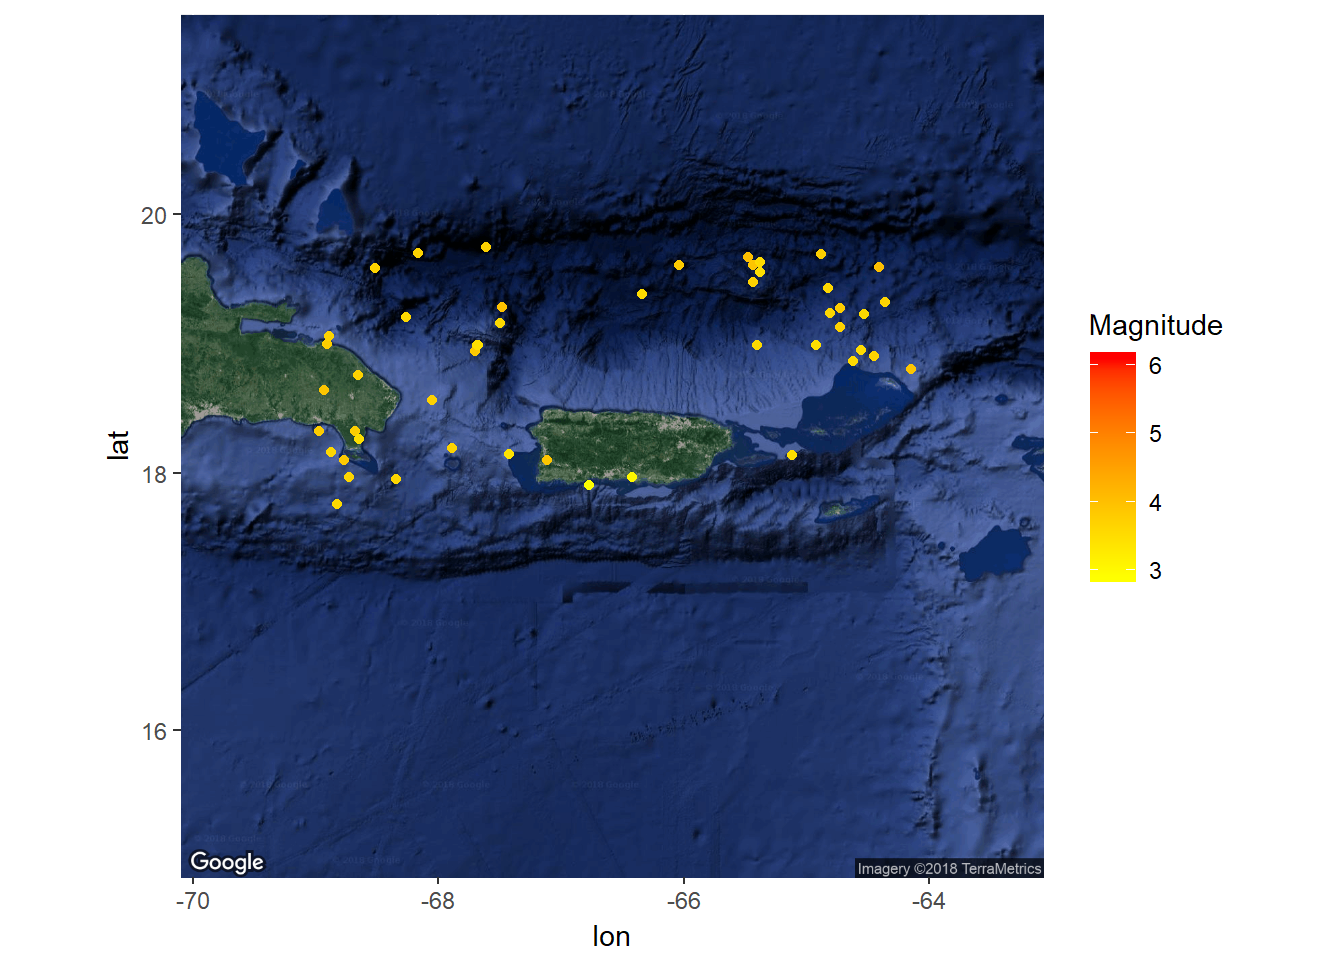
\includegraphics{Homework12_files/figure-latex/unnamed-chunk-2-1.pdf}

\subsection{Lets change some
arguments}\label{lets-change-some-arguments}

\begin{Shaded}
\begin{Highlighting}[]
\CommentTok{# You can also change the zoom, color of the map, color of magnitude scale, size of the dots}
\NormalTok{PRMap2 =}\StringTok{ }\KeywordTok{get_map}\NormalTok{(}\DataTypeTok{location=}\StringTok{'puerto rico'}\NormalTok{, }\DataTypeTok{zoom =} \DecValTok{8}\NormalTok{, }\DataTypeTok{maptype =} \StringTok{"satellite"}\NormalTok{, }\DataTypeTok{source =} \StringTok{'google'}\NormalTok{, }\DataTypeTok{color =} \StringTok{'bw'}\NormalTok{)}
\end{Highlighting}
\end{Shaded}

\begin{verbatim}
## Map from URL : http://maps.googleapis.com/maps/api/staticmap?center=puerto+rico&zoom=8&size=640x640&scale=2&maptype=satellite&language=en-EN&sensor=false
\end{verbatim}

\begin{verbatim}
## Information from URL : http://maps.googleapis.com/maps/api/geocode/json?address=puerto%20rico&sensor=false
\end{verbatim}

\begin{Shaded}
\begin{Highlighting}[]
\KeywordTok{ggmap}\NormalTok{(PRMap2) }\OperatorTok{+}\StringTok{ }\KeywordTok{geom_point}\NormalTok{(}\KeywordTok{aes}\NormalTok{(}\DataTypeTok{x=}\NormalTok{Longitude, }\DataTypeTok{y=}\NormalTok{Latitude, }\DataTypeTok{show_guide =} \OtherTok{TRUE}\NormalTok{, }\DataTypeTok{colour=}\NormalTok{ Magnitude),}
                  \DataTypeTok{data=}\NormalTok{ Earthquakes, }\DataTypeTok{alpha =} \FloatTok{0.99}\NormalTok{, }\DataTypeTok{size=}\DecValTok{3}\NormalTok{, }\DataTypeTok{na.rm=}\OtherTok{TRUE}\NormalTok{) }\OperatorTok{+}\StringTok{ }\KeywordTok{scale_color_gradient}\NormalTok{(}\DataTypeTok{low=}\StringTok{"green"}\NormalTok{, }\DataTypeTok{high =} \StringTok{"black"}\NormalTok{) }
\end{Highlighting}
\end{Shaded}

\begin{verbatim}
## Warning: Ignoring unknown aesthetics: show_guide
\end{verbatim}

\includegraphics{Homework12_files/figure-latex/unnamed-chunk-3-1.pdf}


\end{document}
